\documentclass{ctexart}

%%%%%%%%%%%%%%%%%%%%%%%%%%%%%%%%%%%%%%%%%%%%%%%%%%%%%%%%%%%%%%%%%%%%%%%
%%%%%%%%%%%%%%%%%%%%%%%%%%%%%%%%%%%%%%%%%%%%%%%%%%%%%%%%%%%%%%%%%%%%%%%
%%%%%%%%%%%%%%%%%%%%%%%%%%%%%%%%%%%%%%%%%%%%%%%%%%%%%%%%%%%%%%%%%%%%%%%
%%%%%%%%%%%%%%%%%%%%%%%%%%%%%%%%%%%%%%%%%%%%%%%%%%%%%%%%%%%%%%%%%%%%%%%
%%%%%%%%%%%%%%%%%%%%%%%%%%%%%%%%%%%%%%%%%%%%%%%%%%%%%%%%%%%%%%%%%%%%%%%
\usepackage{hyperref}
\usepackage{amsmath}
\usepackage{setspace}
\usepackage{titletoc}
\usepackage{titlesec}
\usepackage{fontspec}
\usepackage{graphicx}
\usepackage{amssymb}
\usepackage{multirow}
\usepackage{array}
\usepackage{pdfpages}
\usepackage{fancyhdr}
\usepackage{caption}
\usepackage{bicaption}
\usepackage{zhnumber}
\usepackage[a4paper,left=25mm,right=25mm,top=25mm,bottom=25mm]{geometry}
\setmainfont{Times New Roman}

\DeclareCaptionOption{english}[]{%
	\renewcommand\figurename{Figure}%
	\renewcommand\tablename{myTable}%
}
\captionsetup[bi-first]{labelsep=space}
\captionsetup[bi-second]{english,font={stretch=1.25},labelsep=space,name={Fig}}
%\captionsetup[figure]{labelformat={default},,}

\numberwithin{figure}{section}
\numberwithin{table}{section}
\numberwithin{equation}{section}
\captionsetup{labelfont=bf,textfont=bf,font={small}}

%%%%%%%%%%%%%%%%%%%%%%%%%%%%%%%%%%%%%%%%%%%%%%%%%%%%%%%%%%%%%%%%%%%%%%%
%%%%%%%%%%%%%%%%%%%%%%%%%%%%%%%%%%%%%%%%%%%%%%%%%%%%%%%%%%%%%%%%%%%%%%%
%%%%%%%%%%%%%%%%%%%%%%%%%%%%%%%%%%%%%%%%%%%%%%%%%%%%%%%%%%%%%%%%%%%%%%%
%%%%%%%%%%%%%%%%%%%%%%%%%%%%%%%%%%%%%%%%%%%%%%%%%%%%%%%%%%%%%%%%%%%%%%%
%%%%%%%%%%%%%%%%%%%%%%%%%%%%%%%%%%%%%%%%%%%%%%%%%%%%%%%%%%%%%%%%%%%%%%%

\begin{document}

\includepdf{硕士毕业论文封面.pdf}
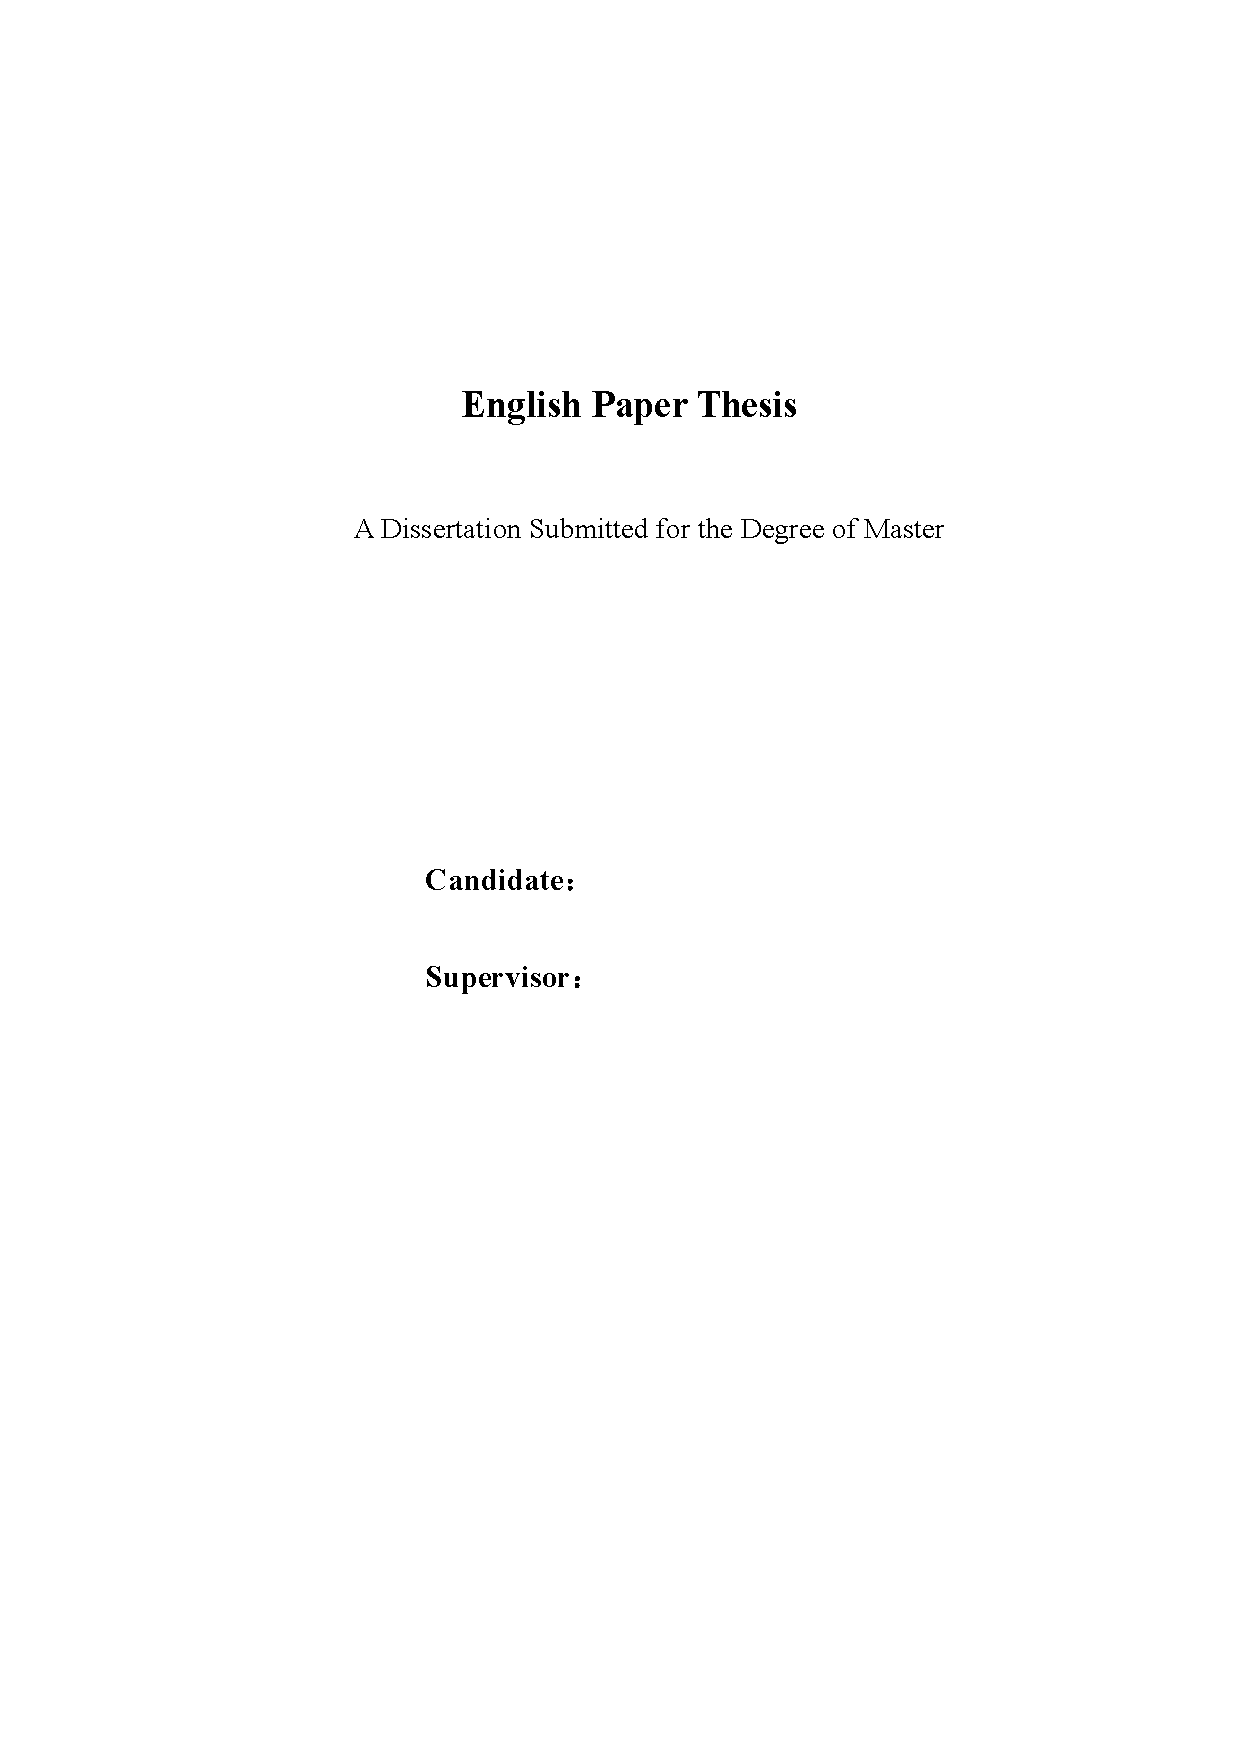
\includepdf{英文封面.pdf}

\includepdf{题名页.pdf}

\includepdf{原创性声明.pdf}
\songti \zihao{-4} \linespread{1.5}
\pagestyle{fancy}
\fancyhf{}
\pagenumbering{Roman}
\fancyfoot[C]{\songti \zihao{5} \thepage}
\renewcommand{\headrulewidth}{0pt}


\renewcommand{\contentsname}{\hspace*{\fill} 目\quad 录\hspace*{\fill}}
\newcommand{\upcite}[1]{\textsuperscript{\cite{#1}}}

\newenvironment{myTable}{\begin{table} \centering \renewcommand\arraystretch{1.15}}{\end{table}}

\makeatletter
\renewcommand{\@maketitle}{
	\begin{center}%
		{\LARGE \@title \par}%
	\end{center}%
	\par} \makeatother
	
\newcommand{\cnabstractname}{摘要}
\newenvironment{enabstract}[1][Abstract]{%
	\begin{center}\zihao{3} \bfseries #1\end{center} %
	\par
	}{\par\vskip 2.5ex}
\newenvironment{cnabstract}[1][摘要]{%
	\begin{center}\bfseries #1 \end{center}%
	\par
}{\par\vskip 2.5ex}
	
%%%%%%%%%%%%%%%%%%%%%%%%%%%%%%%%%%%%%%%%%%%%%%%%%%%%%%%%%%%%%%%%%%%%%%%
%%%%%%%%%%%%%%%%%%%%%%%%%%%%%%%%%%%%%%%%%%%%%%%%%%%%%%%%%%%%%%%%%%%%%%%
%%%%%%%%%%%%%%%%%%%%%%%%%%%%%%%%%%%%%%%%%%%%%%%%%%%%%%%%%%%%%%%%%%%%%%%
%%%%%%%%%%%%%%%%%%%%%%%%%%%%%%%%%%%%%%%%%%%%%%%%%%%%%%%%%%%%%%%%%%%%%%%
%%%%%%%%%%%%%%%%%%%%%%%%%%%%%%%%%%%%%%%%%%%%%%%%%%%%%%%%%%%%%%%%%%%%%%%

\ctexset{
	section={
		format+ = \zihao{3} \songti \setlength{\parskip}{0.5em},
		number=\chinese{section},
		name={第,章 },
	},
	subsection={
		format+ = \zihao{4} \songti,
	},
	subsubsection={
		format+ = \zihao{-4} \songti,
	},
}

\titlespacing{\section}{0pt}{0.5ex plus .0ex minus .0ex}{0.5ex plus .0ex}
\titlespacing{\subsection}{0pt}{0.5ex plus .0ex minus .0ex}{0.5ex plus .0ex}

\hypersetup{hidelinks}

\titlecontents{section}[0pt]{\addvspace{5pt}\filright}              
{\contentspush{\thecontentslabel\ }} 
{}{\titlerule*[8pt]{.}\contentspage}

%%%%%%%%%%%%%%%%%%%%%%%%%%%%%%%%%%%%%%%%%%%%%%%%%%%%%%%%%%%%%%%%%%%%%%%
%%%%%%%%%%%%%%%%%%%%%%%%%%%%%%%%%%%%%%%%%%%%%%%%%%%%%%%%%%%%%%%%%%%%%%%
%%%%%%%%%%%%%%%%%%%%%%%%%%%%%%%%%%%%%%%%%%%%%%%%%%%%%%%%%%%%%%%%%%%%%%%
%%%%%%%%%%%%%%%%%%%%%%%%%%%%%%%%%%%%%%%%%%%%%%%%%%%%%%%%%%%%%%%%%%%%%%%
%%%%%%%%%%%%%%%%%%%%%%%%%%%%%%%%%%%%%%%%%%%%%%%%%%%%%%%%%%%%%%%%%%%%%%%

\begin{cnabstract}
请使用XeLaTex编译
	
\textbf{\zihao{-4} \heiti 关键字:}{\heiti 关键词一, 关键词二...}
\end{cnabstract}
\newpage
\begin{enabstract}[Abstract]
Compile using latex

\textbf{\zihao{-4} Key words:} Key word One, Key word Two...
\end{enabstract}

\newpage

%%%%%%%%%%%%%%%%%%%%%%%%%%%%%%%%%%%%%%%%%%%%%%%%%%%%%%%%%%%%%%%%%%%%%%%
%%%%%%%%%%%%%%%%%%%%%%%%%%%%%%%%%%%%%%%%%%%%%%%%%%%%%%%%%%%%%%%%%%%%%%%
%%%%%%%%%%%%%%%%%%%%%%%%%%%%%%%%%%%%%%%%%%%%%%%%%%%%%%%%%%%%%%%%%%%%%%%
%%%%%%%%%%%%%%%%%%%%%%%%%%%%%%%%%%%%%%%%%%%%%%%%%%%%%%%%%%%%%%%%%%%%%%%
%%%%%%%%%%%%%%%%%%%%%%%%%%%%%%%%%%%%%%%%%%%%%%%%%%%%%%%%%%%%%%%%%%%%%%%

\titlecontents{section}
[3.5em]{\bf \heiti \zihao{-4} \linespread{1.5}}
{\contentslabel{3.5em}}{}{\titlerule*[0.5pc]{$\cdot$}\contentspage}
\titlecontents{subsection}
[3.5em]{\songti \zihao{-4} \linespread{1.5}}
{\contentslabel{2em}}{}{\titlerule*[0.5pc]{$\cdot$}\contentspage}
\titlecontents{subsubsection}
[5em]{\songti \zihao{5} \linespread{1.5}}
{\contentslabel{2.5em}}{}{\titlerule*[0.5pc]{$\cdot$}\contentspage}

\tableofcontents
\newpage
\pagenumbering{arabic}
\setcounter{page}{1}

\fancyhf{}
\fancyhead[C]{\ifodd\value{page}\quad 安徽大学硕士学位论文 \quad\else 第\zhnumber{\thesection}章\quad\leftmark \fi}
\fancyfoot[L]{}
\fancyfoot[R]{}
\fancyfoot[C]{\songti \zihao{5} \thepage}
\renewcommand{\headrulewidth}{0.5pt}


\section{绪论}
\subsection{研究背景}
请使用XeLaTex编译

请使用XeLaTex编译

请使用XeLaTex编译

请使用XeLaTex编译

请使用XeLaTex编译

请使用XeLaTex编译

请使用XeLaTex编译

请使用XeLaTex编译

请使用XeLaTex编译

请使用XeLaTex编译

请使用XeLaTex编译

请使用XeLaTex编译

请使用XeLaTex编译

请使用XeLaTex编译

请使用XeLaTex编译

请使用XeLaTex编译

请使用XeLaTex编译

请使用XeLaTex编译

请使用XeLaTex编译

请使用XeLaTex编译

请使用XeLaTex编译

请使用XeLaTex编译

请使用XeLaTex编译

请使用XeLaTex编译

请使用XeLaTex编译

请使用XeLaTex编译
\subsection{研究内容与创新点}
请使用XeLaTex编译

请使用XeLaTex编译

请使用XeLaTex编译

请使用XeLaTex编译

请使用XeLaTex编译

请使用XeLaTex编译

请使用XeLaTex编译

请使用XeLaTex编译

请使用XeLaTex编译

请使用XeLaTex编译

请使用XeLaTex编译

请使用XeLaTex编译

请使用XeLaTex编译

请使用XeLaTex编译

请使用XeLaTex编译

请使用XeLaTex编译

请使用XeLaTex编译

请使用XeLaTex编译

请使用XeLaTex编译

请使用XeLaTex编译

请使用XeLaTex编译

请使用XeLaTex编译

请使用XeLaTex编译

请使用XeLaTex编译

请使用XeLaTex编译

请使用XeLaTex编译
\subsection{论文的组织架构}
请使用XeLaTex编译

请使用XeLaTex编译

请使用XeLaTex编译

请使用XeLaTex编译

请使用XeLaTex编译

请使用XeLaTex编译

请使用XeLaTex编译

请使用XeLaTex编译

请使用XeLaTex编译

请使用XeLaTex编译

请使用XeLaTex编译

请使用XeLaTex编译

请使用XeLaTex编译

请使用XeLaTex编译

请使用XeLaTex编译

请使用XeLaTex编译

请使用XeLaTex编译

请使用XeLaTex编译

请使用XeLaTex编译

请使用XeLaTex编译

请使用XeLaTex编译

请使用XeLaTex编译

请使用XeLaTex编译

请使用XeLaTex编译

请使用XeLaTex编译

请使用XeLaTex编译
\newpage
\section{相关工作进展}

\subsection{相关工作}
引用英文参考文献\upcite{paper1}。中文参考文献\upcite{paper2}

\newpage
\section{章节标题}
\subsection{引言}

\subsection{模型}
模型的具体框架如图\ref{model_structure}所示。
\begin{figure*}[htbp]
	\centering
	
\includegraphics[width=\textwidth]{模型图.pdf}
	\bicaption{中文标题}{English Title}
	\label{model_structure}
\end{figure*}

模型用到的公式为式\ref{eq}.
\begin{equation}
	O_{i}=CNN_{i}(I_{i}),\qquad i=1,2\cdots z
	\label{eq}
\end{equation}

\subsubsection{小节标题一}

\subsubsection{小节标题二}

\subsection{实验与结果}
实验表格\ref{ablationresult}
\begin{myTable}
	\bicaption{中文表格标题}{English Table Title.}
	\label{ablationresult}
	\begin{tabular}{|c|c|c|c|c|}
		\hline
		类别&指标1&指标2&指标3&指标4\\ \hline
		模型1&0&0&0&0\\ \hline
		模型2&0&0&0&0\\ \hline
		Ours&\textbf{最好的结果加粗}&\textbf{最好的结果加粗}&\textbf{最好的结果加粗}&\textbf{最好的结果加粗}\\ \hline
	\end{tabular}
\end{myTable}



\subsection{分析和讨论}

\subsubsection{讨论一}


\subsubsection{讨论二}

\subsection{本章小结}

\newpage
\section{章节标题}
\subsection{小节标题一}

\subsubsection{次小节标题}


\subsection{小节标题二}

\subsubsection{次小节标题}

\subsection{实验与结果}

\subsection{本章小结}

\newpage
\section{总结与展望}
\subsection{工作总结}

\subsection{工作展望}

\newpage

\fancyhf{}
\fancyhead[C]{\ifodd\value{page}\quad 安徽大学硕士学位论文 \quad\else \leftmark \fi}

\titlecontents{section}
[0em]{\bf \heiti \zihao{-4} \linespread{1.5}}
{\contentslabel{3.5em}}{}{\titlerule*[0.5pc]{$\cdot$}\contentspage}

\addcontentsline{toc}{section}{参考文献}
\bibliographystyle{mybst}
\bibliography{MyBib}
\newpage

%%%%%%%%%%%%%%%%%%%%%%%%%%%%%%%%%%%%%%%%%%%%%%%%%%%%%%%%%%%%%%%%%%%%%%%
%%%%%%%%%%%%%%%%%%%%%%%%%%%%%%%%%%%%%%%%%%%%%%%%%%%%%%%%%%%%%%%%%%%%%%%
%%%%%%%%%%%%%%%%%%%%%%%%%%%%%%%%%%%%%%%%%%%%%%%%%%%%%%%%%%%%%%%%%%%%%%%
%%%%%%%%%%%%%%%%%%%%%%%%%%%%%%%%%%%%%%%%%%%%%%%%%%%%%%%%%%%%%%%%%%%%%%%
%%%%%%%%%%%%%%%%%%%%%%%%%%%%%%%%%%%%%%%%%%%%%%%%%%%%%%%%%%%%%%%%%%%%%%%

\section*{攻读硕士学位期间取得的学术成果}
\titlecontents{section}
[0em]{\bf \heiti \zihao{-4} \linespread{1.5}}
{\contentslabel{3.5em}}{}{\titlerule*[0.5pc]{$\cdot$}\contentspage}
\addcontentsline{toc}{section}{攻读硕士学位期间取得的学术成果}
成果

\newpage
\fancyhf{}
\fancyhead[C]{\ifodd\value{page}\quad 安徽大学硕士学位论文 \quad\else 致谢 \fi}

%%%%%%%%%%%%%%%%%%%%%%%%%%%%%%%%%%%%%%%%%%%%%%%%%%%%%%%%%%%%%%%%%%%%%%%
%%%%%%%%%%%%%%%%%%%%%%%%%%%%%%%%%%%%%%%%%%%%%%%%%%%%%%%%%%%%%%%%%%%%%%%
%%%%%%%%%%%%%%%%%%%%%%%%%%%%%%%%%%%%%%%%%%%%%%%%%%%%%%%%%%%%%%%%%%%%%%%
%%%%%%%%%%%%%%%%%%%%%%%%%%%%%%%%%%%%%%%%%%%%%%%%%%%%%%%%%%%%%%%%%%%%%%%
%%%%%%%%%%%%%%%%%%%%%%%%%%%%%%%%%%%%%%%%%%%%%%%%%%%%%%%%%%%%%%%%%%%%%%%
\section*{致谢}
\titlecontents{section}
[0em]{\bf \heiti \zihao{-4} \linespread{1.5}}
{\contentslabel{3.5em}}{}{\titlerule*[0.5pc]{$\cdot$}\contentspage}
\addcontentsline{toc}{section}{致谢}

	
\end{document}